\section{需求分析与调研}

\subsection{需求分析}

根据题目描述,我们需要实现一个“更加智能的 Flash 文件系统”。

Flash介质因本身的擦除特性,给上层文件系统带来与普通磁盘、内存文件系统不同的数据管理模式。
同时,Flash的写入放大、寿命以及后期稳定性下降等问题也给文件系统的设计带来的一定的挑战。
传统的Flash文件系统并没有很好地解决这些稳定性相关问题。
这里希望寻找一种更智能、更合适的Flash文件系统设计,来更好地平衡Flash的性能与稳定性。
可以思考的方向包括但不限于:数据压缩算法(可以是自适应的压缩算法),检错、纠错、纠删码(可以是联合信源信道编码),数据块选择、擦除策略,Cache机制。

结合赛题内容,我们需要完成的文件系统需要具备以下特性:

\begin{itemize}
  \item {\bf{适合 Flash 介质}}:文件系统需要能够适应并缓解 Flash 的写入放大、寿命、后期稳定性等诸多 Flash 存储介质特有的问题
  \item {\bf{更智能}}:文件系统需要使用多种策略,在软件算法层面平衡性能与寿命
\end{itemize}

\subsubsection{往年实现分析}

本题在去年已经有队伍完成,他们的仓库在 \url{https://gitlab.eduxiji.net/why/project788067-124640}。
在选题之时,我们对其进行了调研。

他们队伍完成了一个基于 UBIFS 的适用于裸 Flash 设备的 YOUBIFS 文件系统,从以下几个方面对其进行了优化:

\begin{itemize}
  \item {\bf{数据压缩模块}}:使用了预压缩和自适应压缩结合的方法,均衡压缩比和写入速度
  \item {\bf{纠错编码模块}}:实现自适应生命周期、CRC+RAID5两种纠错方案
  \item {\bf{Cache 机制}}:添加读写缓冲
  \item {\bf{冷热数据识别}}:使用了冷热识别的纠错以提高 I/O 速度
\end{itemize}

\begin{figure}[htbp]
  \centering
  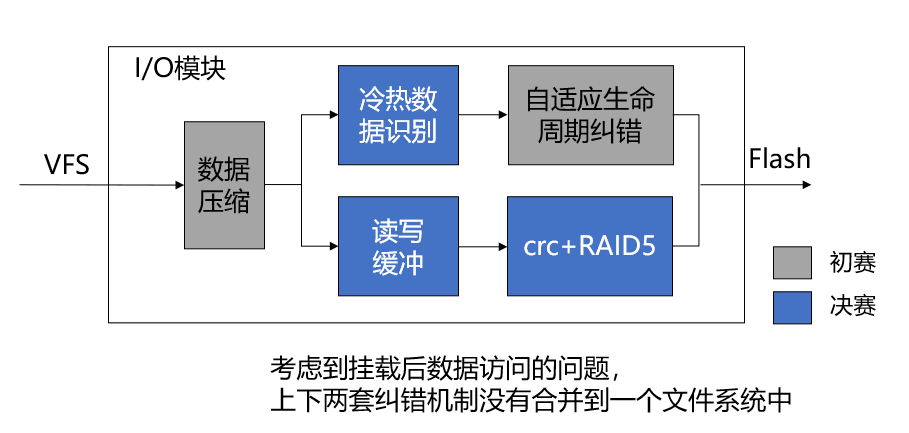
\includegraphics[width=0.7\textwidth]{fig/YOUBIFS项目框图.png}
  \caption{YOUBIFS 系统架构}
  \label{youbifs}
\end{figure}

YOUBIFS 的系统架构如图 \ref{youbifs} 所示。
看起来 YOUBIFS 的实现已经非常满足题目的需求,能够很好地回答题目中提出的几个问题。
但是我们发现,YOUBIFS 的系统实现也存在一些不足之处:

\begin{itemize}
  \item {\bf{Nor Flash 应用场景}}
    
  YOUBIFS 的实现中,文件系统的实现是针对于 Nor Flash 的。
  Nor Flash 在实现上与 Nand Flash 有很大的不同,因此 YOUBIFS 的实现并不能直接应用于 Nand Flash 上,应用场景受到了限制。
  
  同时,Nor Flash 一般用于嵌入式设备,而 Nand Flash 一般用于移动设备或高性能设备,因此 YOUBIFS 的实现也不能直接应用于移动设备或固态硬盘上。
  YOUBIFS 针对于 Nor Flash 的多种写入情况做了优化,但是由于 Nor Flash 的寿命、速度、稳定性等特性,其并不适合在写入负载较高的情况下工作。

  Nor Flash 的寿命一般在 10 万次左右,而 Nand Flash 的寿命一般在 100 万次左右,因此 Nor Flash 广泛用于 BIOS 存储、固件存储等写入负载较低的场景。
  在这些应用场景下,由于存储的数据都是非常重要的系统关键数据,如 Bootloader、系统固件等,因此对于数据的稳定性要求非常高。
  如果系统软件直接在 Nor Flash 上频繁读写,很可能会导致 Nor Flash 的寿命过早耗尽,从而导致系统无法正常启动,造成非常严重的后果,
  所以 Nor Flash 很少用于存储程序运行过程中产生的数据,常见的写入场景为固件更新、系统升级等。

  因此,YOUFIBS 的实现并不能直接应用于移动设备或固态硬盘上,所针对的 Nor Flash 高压写入的应用场景也非常有限。
  这与 YOUBIFS 的各种优化策略相矛盾,因此我们需要重新设计一个适用于 Nand Flash 的文件系统,以扩展更多的应用场景。

  \item {\bf{“智能”,但是还不够智能}}

  YOUBIFS 的实现中,使用了多种策略来平衡性能与寿命,但是这些策略都是相对固定的,只是能够根据不同的情况进行策略切换。
  其中能够体现“智能”的实现有:

  \begin{enumerate}
    \item 通过判断文件名的方式来判断使用的压缩算法和参数,即压缩算法和等级的自适应
    \item 通过检查压缩效果是否合适来判断是否继续压缩,压缩效果不好可能其数据本身就是压缩文件,则再次不压缩
    \item 利用文件系统的 node,判别冷热数据文件
  \end{enumerate}

  为什么说我们认为这些“智能”策略其实还不够智能?
  
  这些策略的优化依据,都是文件系统的当前状态、当前负载请求分类等,没有充分考虑 Flash 的介质特性,如后期稳定性下降和延迟升高等,也没有充分考虑工作负载、实际应用和文件系统的互相配合。也就是说,考虑的因素还是不够多,对 Flash 的针对性优化也不够深入。

  同时,这些策略都是非常简单固定的逻辑。虽然通过参数上的调整,在性能受限制的嵌入式系统中也能够在指定的负载上取得比较好的效果,但是在性能限制不大、更复杂的系统中就很难有出色的表现。这是由策略本身的简单的性质决定的,复杂的系统往往需要更复杂的调整逻辑,而这就需要更加复杂的算法,从简单的逻辑判断到决策树、线性回归、神经网络等,用更加复杂和智能的策略逻辑来适应更加复杂的系统和更高要求的工作环境。

  \item {\bf{测试和展示不够规范}}

  首先是测试环境上的问题。录制的视频中的测试环境是个人计算机,目标设备是计算机上的 SSD 或者内存,而不是项目考虑中的 Nor Flash。

  既然是适用于 Flash 的文件系统,就应该统计和 Flash 相关的数据,从而衡量这个文件系统对 Flash 的稳定性、寿命、速度的综合影响,但是测试中只是在本机上进行了速度的测试,这难以说明问题。为了方便开发和开发过程中的验证,最好应该建立一个 Flash 仿真程序,真正计算在 Flash 中的读写频率、位置等信息,并模拟 Flash 芯片的具体延迟给出具体读写速度。

  其次,对 Flash 芯片的检错、纠错测试也应该基于 Flash 仿真,而不是在内存中写入值。在内存中改变一个或多个字节或比特,可能并不符合实际情况中的数据损坏场景。

  在决赛的文档中,记录了在实际嵌入式场景下在一个 Nor Flash 芯片上运行 YOUBIFS 的相关数据,但是没有体现在录制的展示视频中。演示视频中,不断切换测试脚本和开发环境,并通过切换分支的方式切换功能和版本。这样看视频的人很难看懂在做什么,看懂了也很难说明当前的设计有哪些提升。如果演示的时候就能直观地用自动化脚本生成测试报告,如表格、统计图等,会更加有表现力和说服力。
  没有使用通用的测试脚本或者软件,而是选择自己写脚本测试,难以说明提升。
  测试中大部分测试使用 3~11MiB 大小的连续读写,或者直接使用上百 MiB 的大文件连续读写,这不仅不能说明问题,而且也没有解决实际问题。在复杂的文件读写环境中,大部分读写应该是 4KiB 随机读写,这在其他的文件系统论文中是最重要的指标之一,视频中没有体现。

  \item {\bf{纠错算法和 UBIFS 本身不太兼容}}

  UBIFS 运行在 UBI 层之上,而 UBI 层本身已经做了一层校验和纠错,在上一层遇到一个两个比特级别的错误的可能性并不大,反而是一整块、一整个存储介质完全失效的可能性更高。而 UBIFS 本身的纠错算法是基于比特级别的,这样的纠错算法在 UBI 层已经做了纠错的情况下,就显得多余了。而且,UBIFS 的纠错算法是基于比特级别的,而 UBI 层的纠错算法是基于块级别的,这样的不兼容性也会导致 UBIFS 的纠错算法的效果不好。

  此外,YOUBIFS 中有 CRC+RAID5 的逻辑,但是其只适用于单个 Nor Flash 存储设备,在 UBI 层已经实现校验和纠错的情况下,基于 UBI 层的 YOUBIFS 更应该关注以块或设备为单位的 RAID,而不是以比特为单位的 CRC+RAID。

\end{itemize}

找出这些不足,我们并非为了挑刺,而是为了找到我们的项目前进的方向,摸着石头过河。除了这些不足之处,我们同样研究了前人项目的各种其他特点。

\begin{enumerate}
  \item {\bf{文档量很大:}} 文档中需要包含整个开发流程,需要列举并详细说明涉及到的技术要点和原理,以及配有丰富的示意图和代码段。在前人队伍的文档实现中,很大部分是分析原版 UBIFS 的实现逻辑和代码理解,另外一部分有基于这些理解对技术进行的调研以及自己的实现逻辑。  

  \item {\bf{总代码量很大:}} 原版 UBIFS 的代码量就有 1.5 MiB,所以对代码阅读理解能力也有很高的要求。去除重复文件后,使用 CLOC 统计文件行数如表 \ref{youbifs_code} 所示,队伍自己实现的部分暂未统计。

  \begin{table}
    \centering
  %   \begin{center}
      \begin{tabular}{lcccc}
        \textbf{Language} & \textbf{files} & \textbf{blank} & \textbf{comment} & \textbf{code} \\
        \hline
        C & 48 & 6044 & 12432 & 30124 \\
        C/C++ Header & 13 & 713 & 4033 & 4173 \\
        \hline
        SUM: & 61 & 6757 & 16465 & 34297 \\
      \end{tabular}
  %   \end{center}
      \caption{YOUBIFS 代码统计}
      \label{youbifs_code}
  \end{table}
  
\end{enumerate}

在 YOUBIFS 已经能够完成大部分题目要求的情况下,我们要如何在这个基础上进行改进呢?

依照上面的分析,首先我们可以改变我们文件系统的存储介质。YOUBIFS 使用的是 Nor Flash,那么我们可以选择 Flash 的另一种更加常用更加高性能的品类:Nand Flash。我们的研究基于 Nand Flash,就可以更加贴近实际应用场景,扩展项目的实际用途,也可以更加容易地和其他的文件系统进行对比。

当我们选择基于 Nand Flash 的文件系统,题目需求中的许多方面都出现了新的需求。首先,Nand Flash 的读写单位是页,而 Nor Flash 的读写单位是字节,这就要求我们的文件系统在读写时要考虑到页的边界对齐问题。其次,Nand Flash 之上往往有一层 FTL(Flash Translation Layer),向上隔绝了数据块选择、数据擦除、逻辑物理地址映射等与 Flash 存储介质相关的细节,从而提高了在文件系统层面针对 Flash 进行优化的难度。最后,Nand Flash 的读写速度比 Nor Flash 快,但是擦除速度比 Nor Flash 慢,这就要求我们的文件系统在设计时要考虑到这一点,尽量减少擦除操作的次数。

为了解决这些问题,我们需要对 Nand Flash 的特性进行调研,然后在一种基于 Nand Flash 的文件系统的基础上进行改进。

\subsection{背景调研}

\subsubsection{Flash 的特点和分类}

闪存(Flash Memory)是由日本的 舛岡富士雄 (Fujio Muoka)发明的。他分别于1966年和1971年从日本东北大学(Tohoku University)获得学士和博士学位,博士毕业之后他加入了东芝(Toshiba)公司。在东芝工作期间,他分别于1980年和1988年发明了NOR Flash 和 NAND Flash。

目前市面上的闪存主要有两种:NOR Flash 和 NAND Flash,其分类逻辑和原理如图 \ref {flash-nand-nor} 所示。
一般而言,并行接口的Parallel Flash是基于NOR Flash的;而SSD硬盘,U盘,SD卡,eMMC等通常是基于NAND Flash的。

\begin{figure}[htbp]
  \centering
  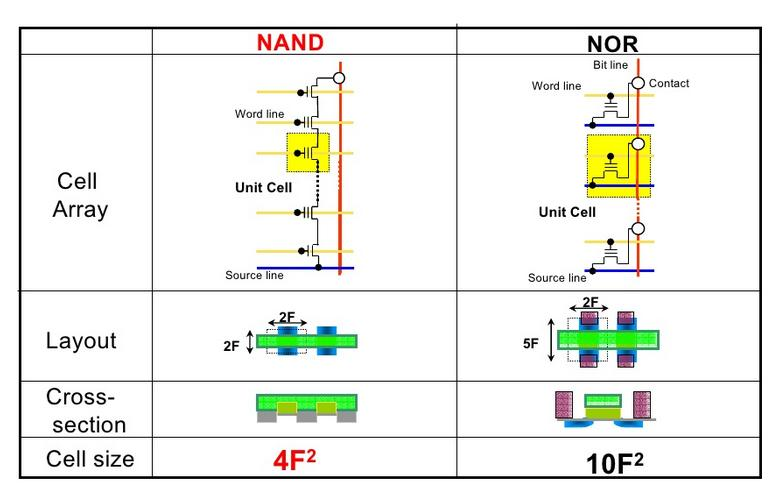
\includegraphics[width=0.85\textwidth]{fig/flash-nand-nor.jpg}
  \caption{Flash 原理与分类}
  \label{flash-nand-nor}
\end{figure}

